\documentclass[11pt]{article}
\usepackage[a4paper,margin=2.5cm]{geometry}
\usepackage[T1]{fontenc}
\usepackage[utf8]{inputenc}
\usepackage{amsmath,amssymb,amsthm}
\usepackage{booktabs,array}
\usepackage{graphicx}
\usepackage{xcolor}
\usepackage[numbers,sort&compress]{natbib}
\usepackage[colorlinks=true,linkcolor=blue!50!black,citecolor=blue!50!black,urlcolor=blue!50!black]{hyperref}
\graphicspath{{../../examples/}}

\newtheorem{proposition}{Proposition}
\newcommand{\qv}{m_v}
\newcommand{\qh}{m_h}

\title{The RBM mutual-information lower bound\\ is fixed by the marginals, not by a learning principle}
\author{Vicente Humberto Monteverde\\
\small Universidad del Museo Social Argentino (UMSA), Argentina\\
\small ORCID 0000-0001-8884-4811}
\date{\small Draft of 27 September 2026}

\begin{document}
\maketitle

\begin{abstract}
A recent review~\cite{singh2026qml} (Sec.~3.2 and Fig.~4 there, after Ref.~[34] of the review)
characterizes a restricted Boltzmann machine (RBM) learner by two numbers for each visible--hidden
pair. The first is the covariance $\eta=\mathrm{Cov}(\sigma_z^v,\sigma_z^h)$, which is read from the
imaginary part of an out-of-time-order correlator. The second is the mutual information $I$. The pair
$(I,\eta)$ is shown to lie between analytic bounds $\mathrm{LB}(\eta)$ and $\mathrm{UB}(\eta)$. Trained
RBMs sit on the lower bound for every system size and field ratio of transverse-field Ising drivers,
and the review reads this as a learning principle: the network would use the least mutual information
compatible with the covariance. We point out that a pair of $\pm1$ units is fixed by three numbers,
the two marginals $m_v=\langle\sigma_z^v\rangle$, $m_h=\langle\sigma_z^h\rangle$ and $\eta$. In those
variables, $\mathrm{LB}(\eta)$ is exactly the case $m_v=m_h=0$, and it is the minimum of $I$ over the
marginals at fixed $\eta$. $\mathrm{UB}(\eta)$ is the perfectly correlated pair with
$|m_v|=|m_h|=\sqrt{1-|\eta|}$. The transverse-field Ising driver is $\mathbb{Z}_2$-symmetric, so a
symmetric RBM has zero marginals and sits on $\mathrm{LB}$ by construction. We test the consequence
that could have failed. With exact enumeration ($n=6$ visible spins, $\alpha=1$), a longitudinal field
of $0.1$--$0.3$ moves the same learner off $\mathrm{LB}$ by up to $0.17$~bits, in step with the
measured marginals. In the ordered phase, a symmetry-broken and a symmetric RBM of the same target sit
off and on $\mathrm{LB}$ respectively. The OTOC reading of $\eta$ is unaffected; we suggest reporting
the marginals alongside $(I,\eta)$.
\end{abstract}

\section{The bounds in terms of the marginals}

For two $\pm1$ variables $s$ (visible) and $t$ (hidden) with marginals $\qv,\qh$ and covariance
$\eta=\langle st\rangle-\qv\qh$, the joint distribution is
\begin{equation}\label{eq:pair}
p(s,t)=\tfrac14\big[1+s\,\qv+t\,\qh+st\,(\eta+\qv\qh)\big],
\end{equation}
and the mutual information (in bits) is
\begin{equation}
I(\qv,\qh,\eta)=h\!\left(\tfrac{1+\qv}{2}\right)+h\!\left(\tfrac{1+\qh}{2}\right)-H(p),
\end{equation}
with $h$ the binary entropy and $H(p)$ the entropy of Eq.~\eqref{eq:pair}. With $\ell(x)=-x\log_2x$, the
bounds of Ref.~\cite{singh2026qml} read $\mathrm{LB}(\eta)=2-2\ell(\tfrac{1+\eta}{4})-2\ell(\tfrac{1-\eta}{4})$ and
$\mathrm{UB}(\eta)=\ell(\tfrac12+\tfrac12\sqrt{1-|\eta|})+\ell(\tfrac12-\tfrac12\sqrt{1-|\eta|})$. Base-2
logarithms reproduce the plotted endpoints $\mathrm{LB}(0)=0$ and $\mathrm{LB}(1)=\mathrm{UB}(1)=1$.

\begin{proposition}
(i) $\mathrm{LB}(\eta)=I(0,0,\eta)$. (ii) $\mathrm{UB}(\eta)=I(r,r,\eta)$ with $r=\sqrt{1-|\eta|}$
(sign of $\qh$ following that of $\eta$), which is the locked pair $t=\pm s$. (iii) To leading order in
$\eta$ and the marginals,
\begin{equation}\label{eq:gap}
I-\mathrm{LB}(\eta)\simeq\frac{\eta^2\,(\qv^2+\qh^2)}{2\ln 2}.
\end{equation}
\end{proposition}
(i) and (ii) follow by substitution into Eq.~\eqref{eq:pair}. For (iii), expand $I$ in the correlation
coefficient $\rho=\eta/\sqrt{(1-\qv^2)(1-\qh^2)}$, using $I\simeq\rho^2/(2\ln2)$. Numerically, on a
grid of marginals, $\mathrm{LB}(\eta)$ is the minimum of $I$ at fixed $\eta$ and $\mathrm{UB}(\eta)$ its
supremum. Eq.~\eqref{eq:gap} is 5\% low at $\eta=0.1$ and 12\% low at $\eta=0.3$. The whole $(I,\eta)$
region is therefore swept by the marginals: at fixed covariance, biased units carry more mutual
information because their variances are smaller (Fig.~\ref{fig:rbm}, left).

\section{Why trained RBMs sit on the lower bound}

The learner's state is the thermal distribution of $H(X)=\sum a_i s_i+\sum b_j t_j+\sum W_{ij}s_it_j$.
The driver $H_{\rm drv}=-B\sum_iX_i-J\sum_{\langle ij\rangle}Z_iZ_j$ commutes with $\prod_iX_i$, so its
ground state has $\langle Z_i\rangle=0$. An RBM with $a=b=0$ is invariant under $(s,t)\to(-s,-t)$, so all
its visible and hidden marginals vanish, and by (i) every pair lies exactly on $\mathrm{LB}(\eta)$.
Saturation of the lower bound is therefore what $\mathbb{Z}_2$ symmetry implies. It is not evidence
that training minimizes mutual information.

This reading makes a prediction that can fail. Break the symmetry, and the points must leave
$\mathrm{LB}$ by the amount Eq.~\eqref{eq:gap} sets from the measured marginals.

\section{Test}

We trained RBM wavefunctions $\psi(v)=e^{a\cdot v}\prod_j2\cosh(b_j+W_j\cdot v)$~\cite{carleo2017} on
the driver with an added longitudinal field $-h_z\sum_iZ_i$. The setup: a periodic chain of $n=6$,
$\alpha=1$, real positive amplitudes (sufficient for this stoquastic driver), exact energy by full
enumeration, L-BFGS, and 3 seeds. For every visible--hidden pair of $P(v,h)\propto e^{a\cdot v+b\cdot
h+v^\top Wh}$ we computed $(\qv,\qh,\eta,I)$ exactly (Table~\ref{tab:rbm}, Fig.~\ref{fig:rbm}, right).

\begin{table}[t]
\centering\small
\caption{Trained RBMs (median over 3 seeds, 36 pairs each). Fidelity is with the exact ground state;
gaps are in bits.}
\label{tab:rbm}
\begin{tabular}{llcccc}
\toprule
$g=B/J$ & $h_z$ & fidelity & $\langle|\qv|\rangle$ & mean $I-\mathrm{LB}$ & max $I-\mathrm{LB}$\\
\midrule
1.0 & 0 & 1.0000 & 0.0001 & $3\times10^{-7}$ & $1\times10^{-5}$\\
2.0 & 0 & 1.0000 & 0.0000 & $7\times10^{-7}$ & $2\times10^{-5}$\\
1.0 & 0.1 & 1.0000 & 0.39 & $1.6\times10^{-2}$ & 0.10\\
1.0 & 0.3 & 1.0000 & 0.52 & $1.4\times10^{-2}$ & 0.17\\
2.0 & 0.1 & 1.0000 & 0.07 & $5.2\times10^{-4}$ & $5\times10^{-3}$\\
2.0 & 0.3 & 1.0000 & 0.18 & $2.7\times10^{-3}$ & $3\times10^{-2}$\\
0.5 & 0 (random start) & 0.50 & 0.81 & $1.1\times10^{-2}$ & 0.12\\
0.5 & 0 ($a=b=0$ start) & 1.0000 & 0.0002 & $1.5\times10^{-8}$ & $1\times10^{-7}$\\
\bottomrule
\end{tabular}
\end{table}

\begin{figure}[t]
\centering
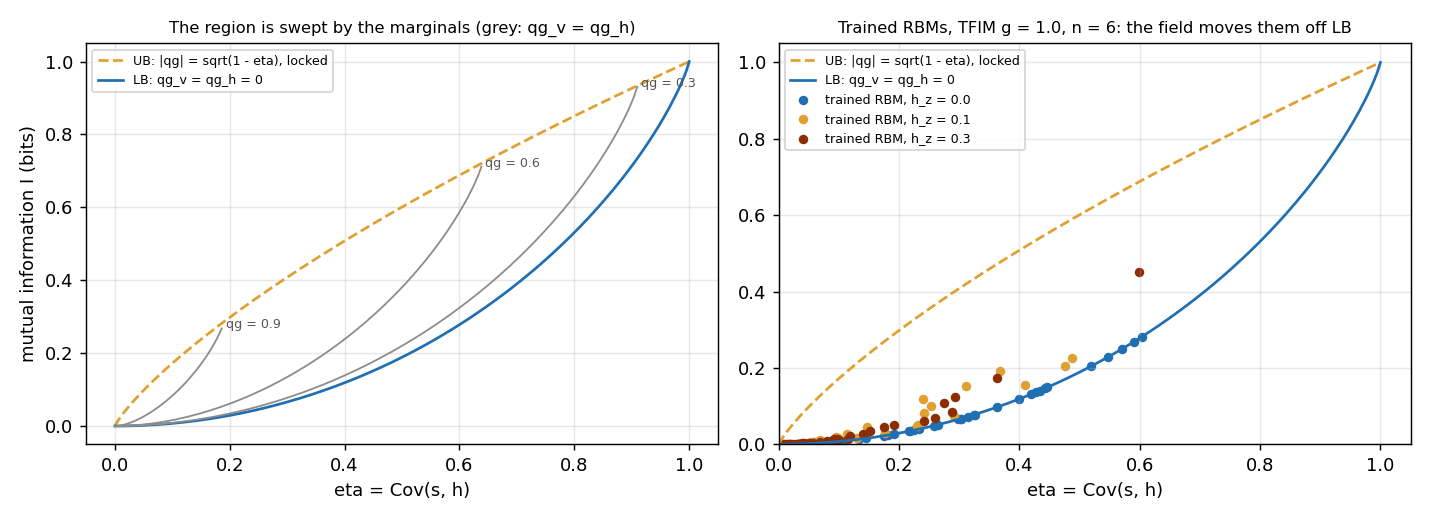
\includegraphics[width=\linewidth]{rbm_mutual_information_qg.png}
\caption{Left: the $(I,\eta)$ region with the bounds of Ref.~\cite{singh2026qml}; grey curves have
fixed marginals $\qv=\qh$. Right: all visible--hidden pairs of trained RBMs at $g=1$ for three
longitudinal fields.}
\label{fig:rbm}
\end{figure}

\begin{itemize}
\item \emph{Symmetric driver.} The review's observation is reproduced: trained RBMs sit on
$\mathrm{LB}$, with gaps below $2\times10^{-5}$~bits, because their marginals vanish.
\item \emph{Broken symmetry.} A field of 0.1--0.3 moves the same learner off $\mathrm{LB}$ by
$5\times10^{-4}$ to $2\times10^{-2}$~bits on average, and up to 0.17~bits for a pair. At $g=2$, where the
marginals are small, Eq.~\eqref{eq:gap} matches the mean gap ($5.3\times10^{-4}$ vs $5.2\times10^{-4}$,
and $2.6\times10^{-3}$ vs $2.7\times10^{-3}$). It underestimates the gap by up to $2\times$ when the
marginals are large.
\item \emph{Same physics, two positions.} In the ordered phase ($g=0.5$) a random start breaks the
symmetry: the fidelity with the symmetric ground state is 0.50 and the marginals are 0.8, and the points
leave $\mathrm{LB}$. A start from $a=b=0$ keeps the symmetry, finds the symmetric ground state exactly,
and the points sit on $\mathrm{LB}$. The target is the same; the position in the $(I,\eta)$ plane is set
by the marginals.
\end{itemize}

\section{Discussion}

The OTOC route to $\eta$ in Ref.~\cite{singh2026qml} and the $(I,\eta)$ picture remain useful. Our
point concerns the interpretation. Lower-bound saturation is the zero-marginal case, and it is fixed by
the symmetry of the driver, or broken by the learner or by a field. It does not require a
minimum-information principle. A simple way to separate the two readings in larger simulations is to
report the marginals $\langle\sigma_z^v\rangle$ and $\langle\sigma_z^h\rangle$ alongside $(I,\eta)$, or
equivalently the distance to $\mathrm{LB}$ predicted by Eq.~\eqref{eq:gap}. A learner that minimized
mutual information would stay on $\mathrm{LB}$ even with $h_z\neq0$; the RBMs here do not.

\paragraph{Limitations.} Our test uses small $n$ with exact enumeration and real RBMs. The
stochastic-reconfiguration training with Monte Carlo sampling at larger $N$ used in the review, and its
long-range driver, are not reproduced. The claim is limited to the one above.

\paragraph{Code availability.} \texttt{examples/rbm\_mutual\_information\_qg.py} and its regression
tests at \url{https://github.com/Viny2030/qang} (MIT license), Sec.~47 of \texttt{RESEARCH\_NOTES.md}.
In the notation of that repository, $\qv$ and $\qh$ are the polar biases $qg_Z$ of the two units, and
$h((1+qg_Z)/2)$ is their $qg_S$~\cite{monteverde2026qang}.

\bibliographystyle{unsrtnat}
\bibliography{../refs}
\end{document}
